\documentclass[twocolumn,10pt]{jarticle}
\usepackage[dvipdfmx]{graphicx}
\usepackage[top=15truemm,bottom=15truemm,left=13truemm,right=13truemm]{geometry}

\title{\vspace{-1.5cm}\normalsize {\textbf {DAOにおける内部告発の提案}}}
\author{\vspace{-1.1cm} \normalsize	情報・通信工学科 荒木研究室所属 182C1117 津田匠貴}
\date{}
\begin{document}
\vspace{-10pt}
\maketitle

%1-----------------------------------------------------------------------------------------------------------
\section{\normalsize はじめに}
\vspace{-0.2cm}
DAO(Decentralized Autonomous Organization:自律分散型組織)は経済的な共通目的を持った匿名個人らが中央集権的な管理主体を持たず
に活動を行う組織であり,独自トークンの発行や分散台帳としての記録機能をもつブロックチェーン技術の使用を前提に成り立っている.
このような組織が運営する分散的サービスはWeb3.0と呼ばれる.これに対し,特定の企業が中央集権的に運営するTwitterなどの従来のサービスはWeb2.0と呼ばれる.
多くのDAOでは自律分散型組織として機能するまでの間,株式会社などの中央集権的組織が主体となって運営している.しかし,彼らによる資金の持ち逃げといった問題が数多く発生している.
不正を防止し,コミュニティによる分散的統治を実現するために,本研究ではEthereumブロックチェーンにおいて秘密分散法を用いたメンバーシップの導入と内部告発機能を提案する.
これは不正を行う兆候があるユーザーを検知した場合に内部告発を行い,メンバーの投票による審議を行うことで,不正を防止するスキームを目指している.

\vspace{-0.1cm}
%2-----------------------------------------------------------------------------------------------------------
\vspace{-0.55cm}
\section{\normalsize 秘密分散法}
\vspace{-0.2cm}
秘密分散法とはある秘密をshareと呼ばれる欠片に分割して,複数のメンバーで管理する方式である.本研究では事前に定めた閾値以上のshareが集まった場合にのみ復元できる閾値型秘密分散法を用いたメンバーシップを提案する.
この手法では,ある多項式上の点をshareとし,それを各メンバーに配布するディーラーの存在を仮定している.閾値以上のshareが集まった場合に多項式を復元することができ,秘密を復号することができる.

%3-----------------------------------------------------------------------------------------------------------
\vspace{-0.55cm}
\section{\normalsize 閾値型秘密分散法を用いたメンバーシップ}
\vspace{-0.2cm}
DAOにおいて内部告発を実現する場合,不正の疑いがあるメンバーを特定する行為は,匿名環境下での活動と矛盾する.
また,内部告発の対象となる資金の持ち逃げは,資金を取り戻すことはほぼ不可能であるため,インシデントが起きる前に不正を防ぐ必要がある.

そのような不正をWeb3.0上の取引から事前に察知するのは困難だが,Twitterなどのチャット内容などから推測できる.そこで,予めこれらのWeb2.0上のアカウントとWeb3.0上のアカウントを紐付けるメンバーシップを考案した.
これにより,告発によってWeb2.0上のアカウントが公開され,メンバーによる判決結果から有害と認められた場合にのみ,被告発者のWeb3.0上のアカウントを特定し罰則を与えることができる.
このスキームでは,不正を行おうとすればリスクを負うため,そのような行いを起こそうとするメンバーに対する牽制や,上述の矛盾を緩和することができる.

\begin{figure}[htbp]
  \begin{center}
    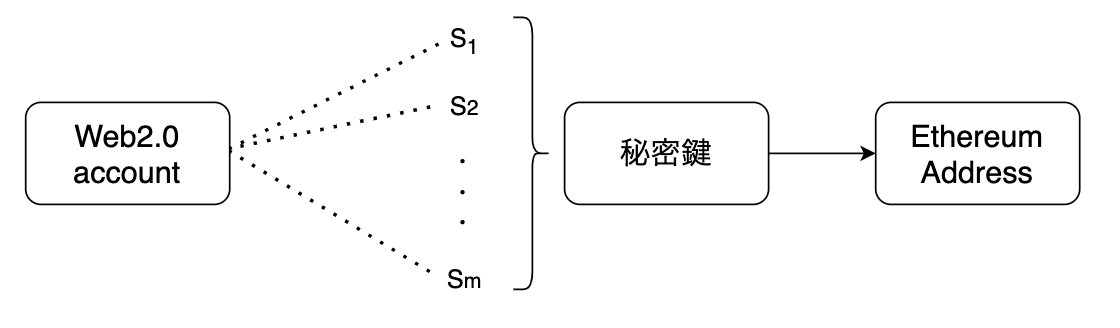
\includegraphics[width=80mm]{share.png}
    \caption{アカウント管理モデル}
  \end{center}
\end{figure}

図1は上述のスキームをEthereum上で実現するために考案したアカウント管理モデルであり,全てのメンバーは以下の流れに従いアカウントを登録する.
\begin{enumerate}
  \vspace{-5pt}
  \item Ethereum Addressを作成する際に使った秘密鍵を$m$個のsecret shareに分割する\vspace{-5pt}
  \item 1つのWeb2.0 accountにつき,$m$個のsecret shareを紐付けたペアを作る\vspace{-5pt}
  \item それぞれのペアを$m$人のメンバーに配る\vspace{-5pt}
\end{enumerate}

これにより,閾値$n$個以上のペアが集まれば,被告発者自身の秘密鍵が復元され,Ethereum Address上の資産を失うなどのリスクを負うことになる.
このようなリスクを回避する唯一の方法は,自身が内部告発の対象にならないことであり,Web2.0上で誠実な振る舞いを続け,DAOに危害を与えるような言動を慎むことである.

%4-----------------------------------------------------------------------------------------------------------
\vspace{-0.55cm}
\section{\normalsize まとめ・今後の展望}
\vspace{-0.2cm}
本研究では,DAOにおけるコアメンバーへの牽制を意図した内部告発スキームの準備としてアカウント管理モデルを提案した.
現在の段階では,ペアの増減に対応できないうえ,中央集権的なディーラーの存在を仮定しているなどの課題がある.そこで,今後はこのような課題を解決できるプロアクティブ秘密分散法を使った改良を行う.
\end{document}
